

\newpage
%%%%%%%%%%%%%%%%%%%%%%%%%%%%%%%%%%%%%%%%%%%%%%%%%%%%%%%%%%%%%%%%%%%%%%%%%%%%%%%%
%%%%%%%%%%%%%%%%%%%%%%%%%%%%%%%%%%%%%%%%%%%%%%%%%%%%%%%%%%%%%%%%%%%%%%%%%%%%%%%%
\section{Dançar na melodia}
\label{subsec:dancamelodia}
\index{Musicalidade!Dançar na melodia}

Como já temos visto até agora sobre os estágios da musicalidade, 
 podemos desenvolver-nos  \hyperref[subsec:dancametrica]{\textbf{dançando na métrica}}  
ou \hyperref[subsec:dancaritmo]{\textbf{dançando no ritmo}};
porém, quando escutamos uma música percebemos que esta não só contem ritmos estruturados, 
com um acento \hyperref[def:Metrica]{\textbf{métrico}}, um \hyperref[sec:pos:timbre]{\textbf{timbre}} 
e uma \hyperref[sec:pos:Intensidade]{\textbf{intensidade}};
se não que também contem \hyperref[sec:pos:Melodia]{\textbf{melodias}} que são compostas, além de outros fatores, 
por mudanças de tons.
Conhecendo isto, 
podemos deduzir que para extrair mais informação da música,
cuja interpretação nos leve a atingir diferentes estilos de dança,
podemos também nos concentrar no aproveitamento de aspectos, relativos à melodia, que não foram tratados 
quando falamos de \hyperref[subsec:dancametrica]{\textbf{dançar na métrica}} ou 
\hyperref[subsec:dancaritmo]{\textbf{dançar no ritmo}}.


Assim, quando escutamos falar sobre dançar na melodia,
geralmente as pessoas não se referem a dançar interpretando as duas principais características de uma melodia,
que são as mudanças de \hyperref[sec:pos:Altura]{\textbf{tom}} e de
\hyperref[sec:pos:Duracion]{\textbf{duração}} nas figuras musicais;
e sim em interpretar estruturas ou aspectos mais complexos de uma melodia (uma voz) na música,
lembrando que esta pode ter uma \hyperref[sec:texturasmusica]{\textbf{textura}} polifônica, monofônica, etc. 


\begin{example}[Percebendo e estudando um poema:]
Para entender um poema poderíamos nos concentrar em estudar as letras, 
espaços em branco  e a posição destes no texto;
porém, estudar desta forma pode ser complexo para um ser humano,
que está acostumado a trabalhar pensando em macro estruturas e não em micro estruturas;
claro que a possibilidade de estudar um poema letra a letra existe,
porém não é isso o que as pessoas geralmente indicam quando dizem que querem estudar uma poesia.
Na forma mais mecânica, 
as pessoas poderiam se referir a estudar as palavras, as frases e sua função no texto;
também a forma em que as frases finalizam em rimas, a métrica,
a velocidade de leitura, entre outros fatores.
Além desta aproximação mais mecânica, 
poderíamos ascender na escala de complexidade e estudar formas ainda superiores de entender a poesia;
por exemplo, baseando-nos em aspectos mais subjetivos como, 
as emoções e sentimentos  que o texto desencadeia em nós;
ou também poderíamos estudar como o texto aumenta e diminui a tensão em nós,
 com o uso adequado das palavras.
\end{example}

Da mesma forma que quando uma pessoa diz que vai estudar um poema, 
não se refere geralmente a estudar ela letra a letra;
quando indicamos que dançaremos na melodia,
não nos referiremos exclusivamente a dançar as mudanças de tom, 
e sim geralmente, se nossa visão da melodia é mais mecânica, que vamos a dançar interpretando os motivos, as frases,
o fraseio, as articulações, as cadencias, as formas estruturais, etc.
Por outro lado se procuramos uma visão e analises mais intimo da melodia,
poderíamos nos referir a interpretar com nossos movimentos, as emoções e sentimentos que a música acorda em nós;
ou poderíamos interpretar a tensão e relaxação que a melodia nos provoca,
também poderíamos incorporar na nossa dança o grau de fluidez ou descontinuidade na articulação das notas musicais, etc.

Assim, observamos que temos vários níveis, 
de onde poderemos extrair características da melodia que possam ser interpretados em nossos movimentos;
a Figura \ref{fig:etapa-melodica-1} mostra de forma ordenada,
algumas características que podem ser extraídas da música, 
agrupados desde estruturas mais complexas (esquerda) a menos complexas (direita).
É importante ressaltar que alguns elementos destes grupos excedem ou divergem da definição de melodia, 
como a textura, a harmonia, etc.
Estos aspectos serão mencionados quando falemos sobre \hyperref[subsec:dancamusica]{\textbf{dançar na música}}.

\begin{figure}[!h]
    \centering
    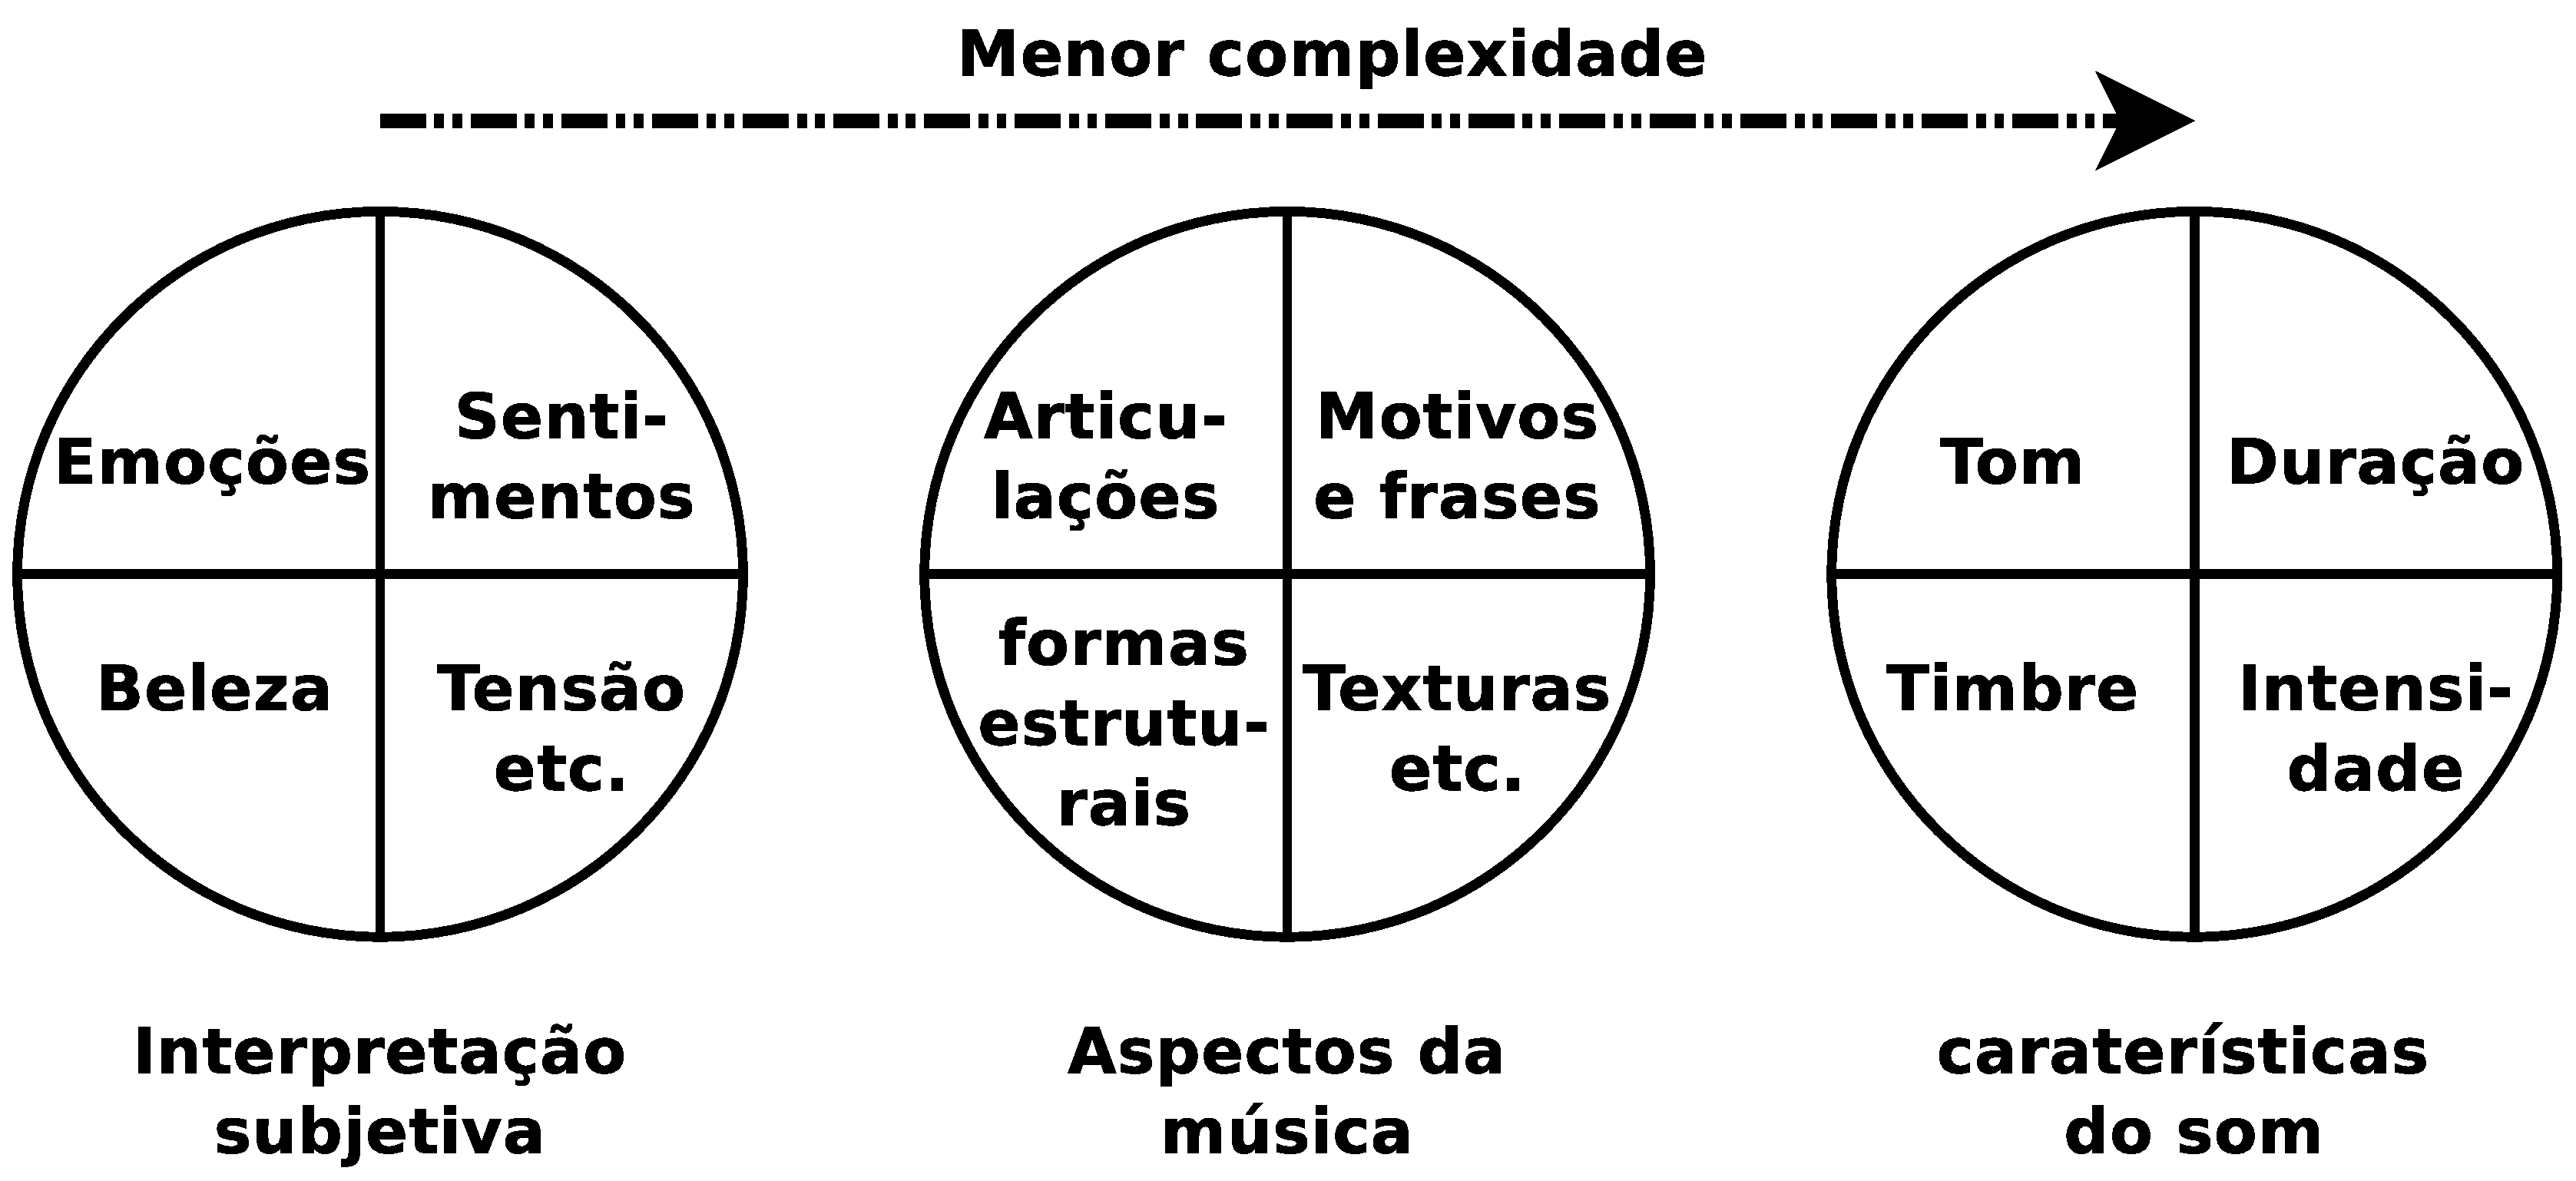
\includegraphics[width=\textwidth]{chapters/cap-musicalidade-tecnica/etapa-melodica-1.eps}
    \caption{Níveis de aproximação à música.}
    \label{fig:etapa-melodica-1}
\end{figure}

Nas seguintes subseções descreveremos como abordar o uso de uma melodia na nossa dança,
seguindo todos os níveis de aproximação à música mostrados na Figura \ref{fig:etapa-melodica-1}.

%%%%%%%%%%%%%%%%%%%%%%%%%%%%%%%%%%%%%%%%%%%%%%%%%%%%%%%%%%%%%%%%%%%%%%%%%%%%%%%%
\subsection{Caraterísticas do som na melodia} 
Na 
Seção \ref{sec:elementosmusica} estudamos as \hyperref[sec:carateristasom]{\textbf{4 características do som}};
a nível de estudo da musicalidade, 
3 destas características já foram aproveitadas quando definimos \hyperref[subsec:dancaritmo]{\textbf{dançar no ritmo}};
sendo estas: 
\hyperref[sec:pos:Duracion]{\textbf{duração}} (ver Exemplo \ref{ex:dancaritmo1}), 
\hyperref[sec:pos:Intensidade]{\textbf{intensidade}} (ver Exemplo \ref{ex:dancaritmo2macro}) e 
\hyperref[sec:pos:timbre]{\textbf{timbre}} (ver Exemplo \ref{ex:danceritmo:bumbopandeiro});
pelo que o aproveitamento destas caraterísticas não será descrito aqui\footnote{\label{footn:melodiatemritmo}Dançar 
na melodia envolve também \hyperref[subsec:dancaritmo]{\textbf{dançar no ritmo}}, 
pois toda melodia tem ritmo; 
porém, nesta seção quando falemos de dançar na melodia, 
só serão abordados aspectos da musicalidade não tratados em estágios anteriores.}.
A este nível de complexidade a única caraterística não usada é 
o \hyperref[sec:pos:Altura]{\textbf{tom}};
ou seja a mudança de \hyperref[sec:pos:Altura]{\textbf{alturas}} nas figuras musicais;
porém, neste ponto devemos ter cuidado, 
pois seguir literalmente as mudanças de tom (altura)
seria mais próximo a \hyperref[subsubsec:musicvisualization]{\textbf{visualização musical}},
 ou a \hyperref[sec:mikeymousing]{\textbf{mickey mousing}}\footnote{Técnicas 
muito boas porém muito fáceis de virar enjoativas se são empregadas desnecessariamente.},
que tem um efeito alegre ou engraçado, e quizas não seja isto o que procuremos.


\begin{example}[Seguindo o tom:] 
\label{ex:musicalidade:melodia:dtons}
Para interpretar as mudanças de tom, 
poderíamos realizar um movimento relativo\footnote{É usada a palavra ``relativo'',
pois não tem necessariamente que ser um movimento ascendente para representar um aumento de tom;
e sim, podemos digerir a ideia e mapear algum outro movimento; 
por exemplo: Aumentar a velocidade quando o tom fique mais agudo.} 
a subir quando o tom aumenta,
e um relativo a descer quando o tom diminui.
\end{example}

Tecnicamente falando, 
fazer um hipotético e literal sobe e desce no Exemplo \ref{ex:musicalidade:melodia:dtons}, 
seria sim dançar na melodia\footnote{Seguir o as mudanças de tom com o corpo, 
de forma literal em todo momento, 
pode levar muito possivelmente a ter uma dança a principio engraçada e logo enjoativa.};
porém, 
existem outras caraterísticas relativas a mudanças de tom na melodia que podemos aproveitar. 

Como já foi estudado da Seção \ref{sec:caracteristicas:melodia},
podemos extrair pelo menos 3 características da melodia,
se analisamos esta em função das mudanças de tom;
estas caraterísticas são:
\{Extensão, Contorno, Movimento\}.
 
\begin{itemize}
\item \textbf{Dançando usando a extensão melódica:}
Melodias com uma \hyperref[ref:melodica:range]{\textbf{extensão melódica}} 
pequena nos produzem geralmente um clima de calma ou quietude;
por outro lado extensões maiores nos produzem geralmente uma sensação de liberdade e expansividade
 \cite[pp. 43]{holland2013music}.
Pelo que, para estar em comunião com a melodia, nossos movimentos deveriam acompanhar estas percepções.
\begin{example}[Usando o rango melódico:]
Na composição musical titulada ``Corcovado''  de Antônio Carlos Jobim,
podemos observar que esta tem uma forma $ABAC$\footnote{Com uma coda de 3 ou 4 compassos, dependendo da versão.},
com seções de 8 compassos binários cada um \cite{partituracorcovado1} \cite[pp. 53]{colluraimprovisacao}.

Ao escutar esta melodia, percebemos que as seções $A$ e $B$ tem uma extensão melódica pequena,
em comparação a seção $C$ que tem uma extensão melódica maior. 
Podemos identificar facilmente a seção $C$, pois a letra que acompanha a seção diz:
``E eu que era triste, descrente desse mundo, ao encontrar você eu conheci ...''.

Assim uma sugestão de interpretação, 
poderia ser usar movimentos com uma extensão pequena e contida para
a seção $A$ e $B$; e movimentos de percorrido mais amplo na seção $C$. 
\end{example}
\item \textbf{Dançando usando o contorno melódico:}
Quando conseguimos perceber o \hyperref[ref:melodica:shape]{\textbf{contorno}} de uma melodia,
podemos usar esta informação para visualizar mentalmente uma curva $f(t)$, em função do tempo $t$;
assim, podemos atrelar $f(t)$ a algum movimento ou \hyperref[sec:musicalidade:dinamicas]{\textbf{dinâmica}}.
\begin{example}[Usando a curva $f(t)$:]
Como já foi adiantado no Exemplo \ref{ex:musicalidade:melodia:dtons},
 os valores $f(t)$ podem ser usados em nossos movimentos; 
a continuação listamos algumas alternativas de uso.
\begin{itemize}
\item Distancia percorrida no salão em função de $f(t)$.
\item O espaço ocupado por nosso corpo ao realizar nossos movimentos em função de $f(t)$.
Por exemplo, se o tom é agudo então usamos um movimento que expanda as pernas, como um ``Romário''
ou um que expanda o espaço do \hyperref[def:Par]{\textbf{par de dança}}, como no ``assalto'', 
e se o tom é grave poderíamos usar movimentos no lugar usando um 
\hyperref[def:abracodedanca]{\textbf{abraço de dança}} fechado. 
\item \hyperref[subsec:dinamica:velocidade]{\textbf{Velocidade}} de nossos movimentos 
em função de $f(t)$, ver Figura \ref{fig:mapeamento-melodica-ft}.
\item \hyperref[sec:musicalidadetensionrelease]{\textbf{Tensão e relaxação}} de nosso corpo em função de $f(t)$.
\item etc.
\end{itemize}
Além de todas estas possibilidades, poderíamos fazer combinações e intercalar ou uso  destas escolhas.
\end{example}
\begin{figure}[!h]
    \centering
    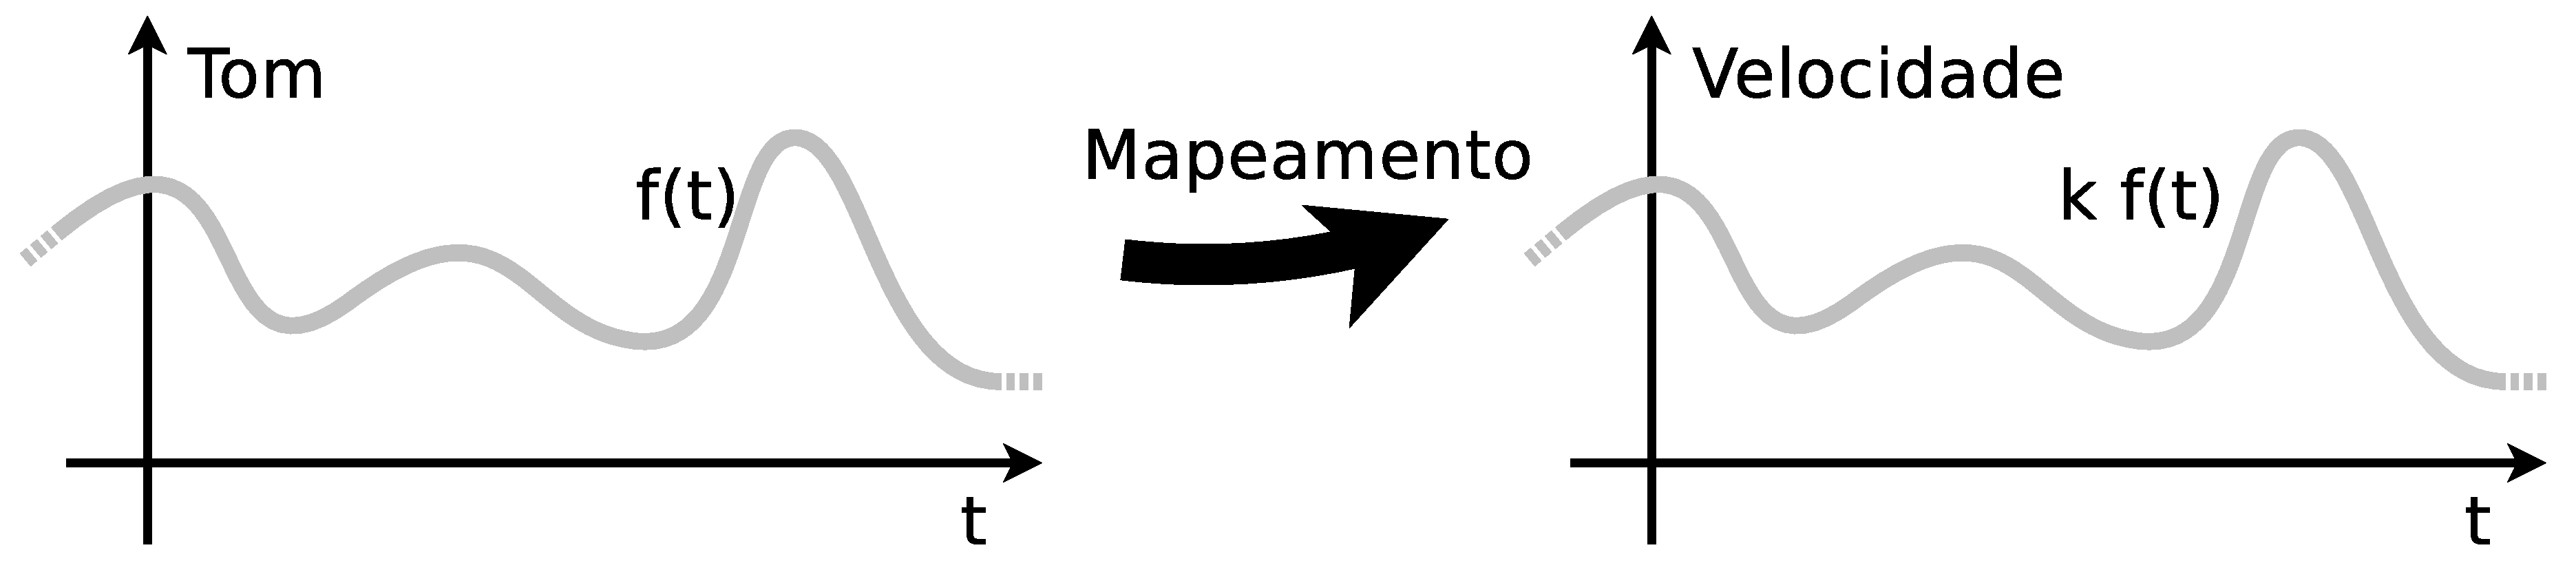
\includegraphics[width=0.9\textwidth]{chapters/cap-musicalidade-tecnica/ft.eps}
    \caption{Contorno melódico mapeado a velocidade, onde $k$ é uma constante.}
    \label{fig:mapeamento-melodica-ft}
\end{figure}

\item \textbf{Dançando usando o movimento melódico:}
Quando vimos o tema da \hyperref[ref:melodica:range]{\textbf{extensão melódica}},
quantificamos às melodias em função da distancia entre a nota musical mais alta e a mais baixa;
este critério nos deu a possibilidade de projetar nossa dança entre dois extremos,
livre e contido, respetivamente;
porém este tipo de avaliação é um parecer promédio,
para a melodia ou uma porção dela. 
Assim, se escolhemos um movimento como deslocar-nos numa direção 
para interpretar a \hyperref[ref:melodica:range]{\textbf{extensão melódica}} numa porção de melodia,
observaremos que precisamos de um critério que nos indique como serão os sub-movimentos para completar esta ação;
este critério pode ser completado se usamos o analises do \hyperref[ref:melodica:movimento]{\textbf{movimento melódico}},
para escolher as \hyperref[sec:musicalidade:dinamicas]{\textbf{dinâmicas}} dos submovimentos.
\begin{example}[Usando o movimento melódico:]
Se percebemos que a melodia esta composta por 
\hyperref[ref:melodica:movimento:conjunto]{\textbf{movimentos melódicos conjuntos}};
então, 
os sub-movimentos de nossa dança poderiam ser executados realizando mudanças pequenas ou deslocamentos curtos,
por outro lado se percebemos \hyperref[ref:melodica:movimento:disjunto]{\textbf{movimentos melódicos disjuntos}},
os sub-movimentos de nossa dança poderiam ser executados realizando mudanças grandes ou deslocamentos longos.
\end{example}
\end{itemize}


 
%%%%%%%%%%%%%%%%%%%%%%%%%%%%%%%%%%%%%%%%%%%%%%%%%%%%%%%%%%%%%%%%%%%%%%%%%%%%%%%%
\subsection{Aspectos da música na melodia} 
Quando analisamos a música desde um ponto de vista mais técnico, 
podemos extrair desta varias caraterísticas; 
neste sentido, nos Capítulos \ref{cap:musicabasica},
\ref{cap:musicacomposer} e \ref{cap:musicatopicos},
foram apresentadas algumas características da música, 
descritas desde o ponto de vista do compositor musical;
por outro lado, no Capítulo \ref{cap:percepcaomusical} 
foram abordados alguns aspectos da música desde o ponto de vista da percepção de um ouvinte.
Assim, juntando estas duas visões da música,
podemos formar um critério para interpretar  na nossa dança um componente da música, como a melodia.

A seguir listaremos algumas sugestões sobre escolhas criativas para interpretar a melodia na nossa dança,
com esse motivo são propostas \hyperref[sec:musicalidade:dinamicas]{\textbf{dinâmicas}} para ser executadas sobre aspectos da música na melodia. 
\begin{itemize}
\item \textbf{Motivos condutor (leitmotiv):} Como é explicado em profundidade na Seção \ref{sec:leitmotivdanca}
o \hyperref[sec:leitmotivdanca]{\textbf{leitmotiv}} é um tema musical básico e 
breve que se repete sempre que se encena algo relacionado a uma personagem, 
situação ou ideia simbólica.
\begin{example}[Leitmotiv de Superman:] Quando num filme ``Superman'' sai numa cena, geralmente no 
fundo se escuta um piano tocando 4 ou 5 notas representativas para o personagem de ``Superman''. 
\end{example}
O \hyperref[sec:leitmotivdanca]{\textbf{leitmotiv}} se acha facilmente no cinema e na opera, 
mas é menos comum na música popular, porém isso não quer dizer que não possamos aproveitar esse recurso,
pois quando dançamos nós somos a personagem em cena e podemos escolher algum motivo 
musical para ser o leitmotiv de algum passo ou movimento nosso.
\begin{example}[Brincando com o pião:]
Na música ``Gostoso veneno'' interpretado por  Alcione e Djavan, 
podemos criar um leitmotiv com as palavras veneno e envenena,
de modo que realizaremos, por exemplo, um pião sempre que se fale alguma destas palavras.
Assim, o veneno seria o leitmotiv do pião.
\end{example}  
No caso anterior
foi escolhida uma palavra cantada como leitmotiv 
pela facilidade em que esta pode ser reconhecida, porém poderia ser usado
um motivo qualquer, por exemplo, um executado de forma instrumental.
\item \textbf{Motivos ou ideias melódicas:} Neste caso podemos escolher um motivo, 
ou uma pequena ideia melódica e aplicar uma dinâmica em concordância com esta ideia melódica
quando a reconhecemos no transcurso de nossa dança. 
É conveniente que essa atribuição seja relativa ao som escutado, ou seja 
se o motivo é triste, alegre, com tensão ou relaxado nosso movimento escolhido deve evidenciar esta característica
\begin{example}[Usando motivos:]
Na música ``Aquarela do Brasil'' interpretada por Alexandre Pires, 
existe um motivo que é executado 4 vezes ao inicio da música, 
só com pequenas variações cada vez. 
Usando esta característica podemos realizar variações de pica-pau ou escovinhas em cada execução do motivo. 
\end{example}  
\item \textbf{Cadências nas frases:} Neste ponto podemos interpretar
os finais masculinos e femininos nas frases musicais  e  
os tipos de \hyperref[sec:Cadencia]{\textbf{cadências}}
(frases tem cadências 
\hyperref[subsec:cadenciamelodica]{\textbf{melódicas}} e 
\hyperref[sec:CadenciaHarmonica]{\textbf{harmônicas}})   
que \hyperref[subsec:FinalAbertoFechado]{\textbf{subjetivamente nos dão a sensação}} 
de uma frase incompleta e de final insatisfatório ou um final completo e satisfatório, como é visto na Seção \ref{subsec:FinalAbertoFechado}.
Assim, nós podemos interpretar esses finais com movimentos que evidenciem 
essas percepções.
\begin{example}[Usando cadencias nos breques:]
Na música ``Eu sou a marrom'' interpretada por Alcione existem breques sincopados
que dão a sensação de surpresa, podemos acompanhar estes finais de frase executando movimentos 
com um enfases que evidencie esta surpresa. Por exemplo com um movimento abrupto 
que de a sensação que tropeçamos e caímos no breque. 
\end{example}  
Na Seção \ref{sec:percepcionbreak} podemos ver mais detalhes de como perceber os breques nas músicas.
\item \textbf{Fraseio da linha melódica:} Podemos empacotar nossos movimentos em frases ``coreográficas''
que acompanhem as frases musicais, para reconhecer as frases na música faremos uso da melodia (ritmo e mudanças de tom),
como já foi adiantado nos Exemplos \ref{ex:dancaritmo1macro} e \ref{ex:dancaritmo2macro},
nós podemos usar a parte rítmica de uma melodia para identificar frases musicais,
porém usar nossa percepção das mudanças de tom nas melodias nos ajudará a identificar melhor 
os finais e inícios de frases musicais.
\begin{example}[Usando frases de 8 tempos:] Para afinar nossa percepção das frases musicais
podemos usar músicas com um constante comprimento de frase.
As seguintes músicas tem frases regulares de 8 tempos:
\begin{itemize}
\item ``Piston da gafieira'' interpretado por Moreira da Silva.
\item ``Tamborim'' interpretado por Clube do Balanço.
\item ``Suingue de samba'' interpretado por Rogê.
\end{itemize}
Para realizar nosso treinamento podemos escolher dois tipos de movimentos, como o cruzado e o balanço,
e usar um destes movimentos numa frase musical e outro na seguinte, 
se para nós é mais fácil identificar as frases contando 
os tempos, então ao principio pode ser feito assim, mas o alvo do exercício é identificar as frases 
de forma mais geral usando vários aspectos como a cadências, 
tensão e relaxação nas frases, motivos, tempos forte e fracos, etc. 
\end{example} 
\item \textbf{Articulações:} Uma alternativa para enriquecer nossa dança é
interpretar com nossos movimentos como são executadas as transições de tom 
(\hyperref[sub:Articulation]{\textbf{articulações}}).
Por exemplo na Seção \ref{subsec:continuidade:ls} é mostrado como interpretar
as melodias quando as mudanças de tom são continuas ou abruptas. 
\item \textbf{Formas estruturais:}
Podemos empacotar nossos movimentos em seções de modo que estas
acompanhem a estrutura da música.
\begin{example}[Partes da música:]
Em muitas ocasiões, além de reconhecer frases na música,
podemos reconhecer estruturas superiores como\footnote{Para mais detalhes ir a Seção\ref{subsec:partesmusica}.}
a \hyperref[ref:Introducao]{\textbf{introdução}},
o \hyperref[ref:Verse]{\textbf{verso}},
a \hyperref[ref:Ponte]{\textbf{ponte}},
o \hyperref[ref:Coro]{\textbf{coro}}, e
a \hyperref[ref:Coda]{\textbf{coda}}.
Assim, quando dançamos podemos atribuir um conjunto diferenciado de movimentos
a cada uma de estas partes. 
Por exemplo um movimento leve na introdução, um movimento regular no verso, 
algo empolgante no coro e um grande final na coda.
\end{example}
Em algumas ocasiões para nós pode ser difícil reconhecer se algo é um coro, uma ponte o um verso,
porém observamos que uma parte da músicaé diferente de outra e reconhecemos que a música 
está dividida em várias partes que se repetem em alguma sequencia;
isto é assim porque como vimos na Seções \ref{sec:FormaMusical} e \ref{sec:compondoestruturadamente}
a música pode e geralmente é composta de forma modular.
Nesses casos podemos tomar uma abordagem como no seguinte exemplo.
\begin{example}[A forma da música:]
Se reconhecemos que numa música temos seções diferenciadas, que chamaremos $A$, $B$, $C$, etc.
tentaremos identificar se a música tem\footnote{Para mais detalhes da forma da música ir a Seção \ref{sec:FormaMusical}.}
\hyperref[subsec:formabinaria]{\textbf{forma binária ($AB$)}}, 
\hyperref[subsec:formaternaria]{\textbf{forma ternária ($ABA$)}}, 
\hyperref[subsec:formarondo]{\textbf{forma rondó ($ABACA$)}},  
\hyperref[subsec:formaabac]{\textbf{forma $\mathbf{ABAC}$}}, 
etc.
A partir desse conhecimento escolheremos um conjunto diferenciado de movimentos para cada seção. 
\end{example}
\end{itemize}



%%%%%%%%%%%%%%%%%%%%%%%%%%%%%%%%%%%%%%%%%%%%%%%%%%%%%%%%%%%%%%%%%%%%%%%%%%%%%%%%
\subsection{Percepção subjetiva da melodia} 
Na verdade o título da seção deveria ser uma percepção ``mais'' subjetiva da melodia,
pois toda interpretação tem algum nível de subjetividade. 
Nesta seção serão dadas algumas indicações para trabalhar uma aproximação à dança 
orientada a explorar o como aspectos de nosso mundo interno
são levados ao mundo externo mediante nossa própria singularidade.
Tendo isso em consideração, a continuação são listados alguns conselhos relevantes quando dançamos com a melodia.
\begin{itemize}
\item Precisaremos nos concentrar na qualidade da expressão emocional da linha melódica na nossa dança,
isto é, se a música nos evoca alegria, entusiasmo, surpresa, tristeza, etc. nossos movimentos
devem transmitir informação em comum com essas percepções.

\item Uma melodia não pode existir sem ritmo, 
as mudanças de tom sobre um ritmo acrescentam emoção, doçura e continuidade à melodia.
Assim, uma forma de aproveitar as informações na melodia é acrescentar a nossos movimentos, 
baseados no ritmo,
uma roupagem\footnote{Uma forma de fazer isto é aplicando \hyperref[sec:musicalidade:dinamicas]{\textbf{dinâmicas}}.} proveniente de nossa percepção subjetiva.


\item O uso de informação da melodia na nossa dança provoca que nossos movimentos se tornem elegantes, 
graciosos e com sentimento, pois para um observador de nossa dança é fácil perceber a beleza, emoção e fluidez da melodia.
Como se pude-se ouvir com os olhos.
\end{itemize}

Além dos comentários anteriores, gostaria agregar uma experiencia pessoal,
pois quando escuto uma música por primeira vez, 
de forma livre e descompromissada de aspectos teóricos, 
as mudanças na melodia  são difíceis de prever para mim.
Por exemplo, algumas vezes eu escuto um motivo musical o qual me provoca um sentimento agradável e aconchegante,
e me nasce executar um movimento como o puladinho, pois sinto nesse momento que ele encaixa bem com essa ideia,
porém de repente a melodia inicia a acelerar e eu não consigo acompanhar coerentemente 
as mudanças da melodia com meus movimentos.
Nesses casos eu tento treinar meu improviso para conseguir mudar de movimento, a algum que encaixe melhor com a nova 
proposta da melodia, mas aqui nasce outro problema, 
se nosso vocabulário de passos ou movimentos de dança é limitado, 
então pode ser difícil achar um movimento que encaixe na melodia,
por outro lado se nossa agilidade mental não é suficiente,
muitas vezes saberemos que movimento queremos fazer porém 
não saberemos nesse momento como executar-lho ou quando descobrimos como fazê-lo a melodia já mudou novamente.
Assim, para todos esses problemas o remédio que me imponho é o treino.



%%%%%%%%%%%%%%%%%%%%%%%%%%%%%%%%%%%%%%%%%%%%%%%%%%%%%%%%%%%%%%%%%%%%%%%%%%%%%%%%
\subsection{Exemplos} 

Finalmente, usando todo o mencionado nas seções anteriores, podemos fazer o seguinte exercício.
\begin{example}[Usando as mudanças de tom:] De forma unipessoal, 
treinaremos o aprovetamento da melodia evitando tomar informação da parte rítmica, 
pois em este caso tentaremos aproveitar em maior medida a informação das mudanças de tom,
com este fim nossas pisadas estarão limitadas a ser executadas num ritmo continuo (em tempo),
ou sem ritmo (pausa), 
isto é nos só temos duas opções: mexer os pés em tempo ou não deslocar os pés. 
Assim, obrigaremos a nosso cérebro a gerar riqueza em nossos movimentos mediante a extração de informação das 
mudanças de tom na melodia.
Para interpretar estas mudanças de tom aplicaremos 
\hyperref[sec:musicalidade:dinamicas]{\textbf{dinâmicas}} a nossos movimentos.
Algumas músicas que podemos usar para treinar o aproveitamento das mudanças de tom são:
\begin{itemize}
\item ``Balanço Zona Sul'' interpretado por Glaucia Nasser.
\item ``Meu caro amigo'' interpretado pelo Grupo Vou Vivendo.
\item ``Choro esdrúxulo'' interpretado por Jards Macalé.
\item ``Nada é impossível'' interpretado pelo Grupo Magia.
%\item ``Pra nunca mais ter fim'' interpretado pelo Grupo Magia.
\item ``Delírios de amor'' interpretado por Alcione.
\item ``Mais além'' interpretado por Alexandre Pires.
%\item ``Tira ela de mim'' interpretado por Alexandre Pires.
\item ``Meu lugar'' interpretado por Arlindo Cruz.
\item ``É com esse que eu vou'' interpretado por Elis Regina.
\end{itemize} 
\end{example}
